\documentclass[11pt]{article}

\usepackage{amssymb}
\usepackage{amsmath}
\usepackage{xcolor}
\usepackage{graphicx}

\usepackage{placeins}
\usepackage{hyperref}

\graphicspath{ {images/} }

\setlength\parindent{0pt}

\begin{document}

\title{Model Predictive Control notes}
\author{Philippe Weingertner}
\date{\today}
\maketitle

\tableofcontents

\section{Motion Control}

Motion Control deals with the last stage of an autonomous driving pipeline: the control module.
The input to the control module will be provided by the output of the path planning module via a set of waypoints to follow as close as possible.
The control module will have to provide the actuators commands (in our case steering angle and throttling; acceleration or deceleration) so that the automated driving comply with a set of rules:


\begin{itemize}
\item follow the planned waypoints as close as possible
\item drives smoothly
\item try to adjust the speed: as fast as a configurable reference when possible and driving more slowly during curves
\end{itemize}



\begin{figure}[h]
    \centering
    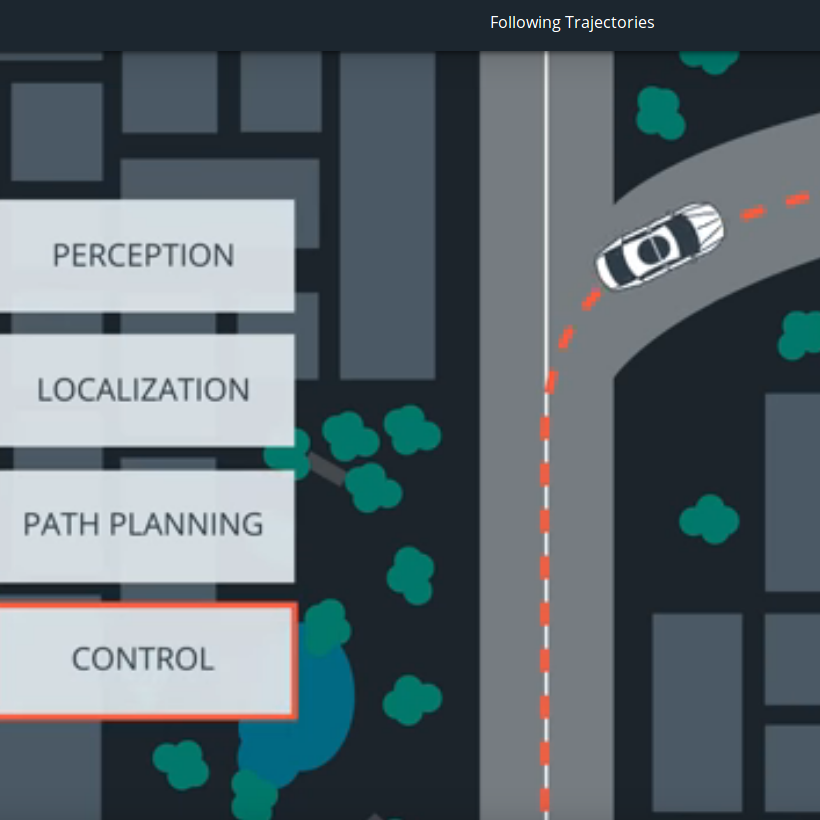
\includegraphics[width=0.5\textwidth]{pipeline}
    \caption{Autonomous Driving pipeline}
    \label{fig:pipeline}
\end{figure}

\section{Non linear optimization under constraints}

\subsection{Definition}

In its most generic form we are dealing with the following problem:

\begin{equation*}
\begin{aligned}
& \underset{x}{\text{minimize}}
& & f_0(x) \\
& \text{subject to}
& & lower_i \leq f_i(x) \leq upper_i, \; i = 1, \ldots, m.
\end{aligned}
\end{equation*}

Note that by setting $lower_i = upper_i $ we can define constraints as equalities as well.

\subsection{Example}

\begin{equation*}
\begin{array}{lc}
{\rm minimize \; }      &  x_1 * x_4 * (x_1 + x_2 + x_3) + x_3 \\
{\rm subject \; to \; } &  x_1 * x_2 * x_3 * x_4  \geq 25 \\
                        &  x_1^2 + x_2^2 + x_3^2 + x_4^2 = 40 \\
                        &  1 \leq x_1, x_2, x_3, x_4 \leq 5
\end{array}
\end{equation*}

\subsection{Solving with ipopt}

ipopt and cppad are used to solve non-linear minimization problems.
ipopt requires the computation of first order (Jacobians) and 2nd order derivatives (Hessians).
These derivatives will be computed automatically thanks to cppad: providing automatic differentiation services. \\
The previous example is solved with ipopt and CppAD here:
\url{https://www.coin-or.org/CppAD/Doc/ipopt_solve_get_started.cpp.htm}

\section{Vehicle Models}

\subsection{Dynamic vs Kinematic Models}

\subsection{Kinematic Model}

\subsubsection{State}

The state variables are the following:

\begin{figure}[h]
    \centering
    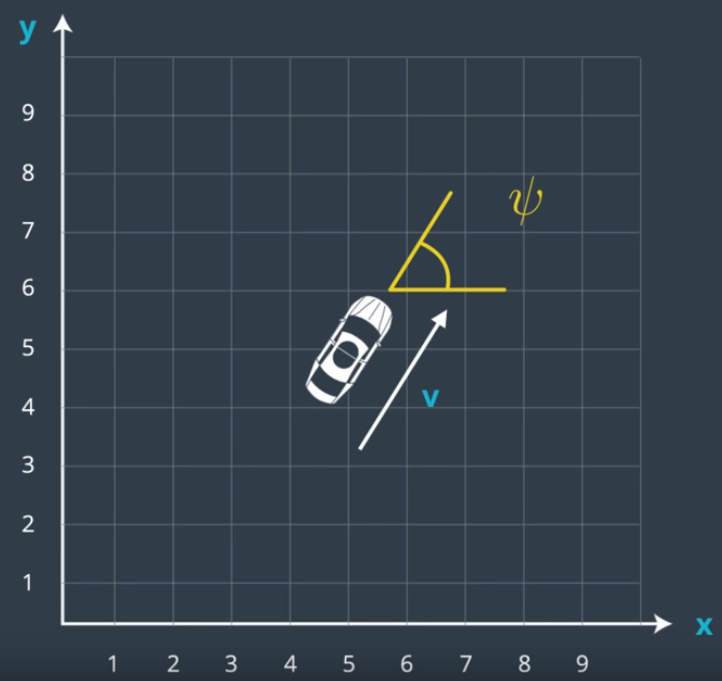
\includegraphics[width=0.5\textwidth]{state}
    \caption{Model state}
    \label{fig:state}
\end{figure}
\FloatBarrier

\begin{itemize}
\item $x$: x position
\item $y$: y position
\item $\psi$: angle between speed vector and x-axis
\item $v$: speed vector
\end{itemize}

\subsubsection{Deriving the kinematic model}


Our state vector is $$ S_t = [x_t, y_t, \psi_t, v_t] $$

We derive an approximation model, kinematic, relating $S_{t+1}$ and $S_t$. The smaller the $dt$ the more accurate the model. \\

\textbf{Linear movement approximation}: assuming during $dt$ that $v_t$ and $\psi_t$ are constant:
$$ x_{t+1} = x_t + v_t * \cos(\psi_t) *  dt $$
$$ y_{t+1} = y_t + v_t * \sin(\psi_t) *  dt $$

\textbf{Rotational movement approximation}: assuming during $dt$ that $v_t$ and steering angle $\delta_t$ are constant:

$$ {M_{t+1}M_{t}} = \rho * (\psi_{t+1} - \psi_t) = v_t * dt$$
$$ \tan(\delta_t) = L_f / \rho $$
So we have:
$$ \psi_{t+1} = \psi_t + (v_t /\rho) * dt$$
$$ \psi_{t+1} = \psi_t + (v_t / L_f) * \tan(\delta_t) * dt $$
\textit{Note that for small $\delta_t$ we have $\tan(\delta_t) \approx \delta_t$} \\

\textbf{Speed update}: assuming during $dt$ that $a_t$ is constant:
$$ v_{t+1} = v_t + a_t * dt $$ \\

So to summarize our kinematic model is:

$$ x_{t+1} = x_t + v_t * \cos(\psi_t) *  dt $$
$$ y_{t+1} = y_t + v_t * \sin(\psi_t) *  dt $$
$$ \psi_{t+1} = \psi_t + (v_t / L_f) * \tan(\delta_t) * dt $$
$$ v_{t+1} = v_t + a_t * dt $$

The state vector is $ S_t = [x_t, y_t, \psi_t, v_t] $. \\
The actuator command $ A_t = [ a_t, \delta_t ] $ defines a \textbf{constraint} between $S_{t+1}$ and $ S_t $.


\subsubsection{Errors}

The errors variables are the following:
\begin{figure}[h]
    \centering
    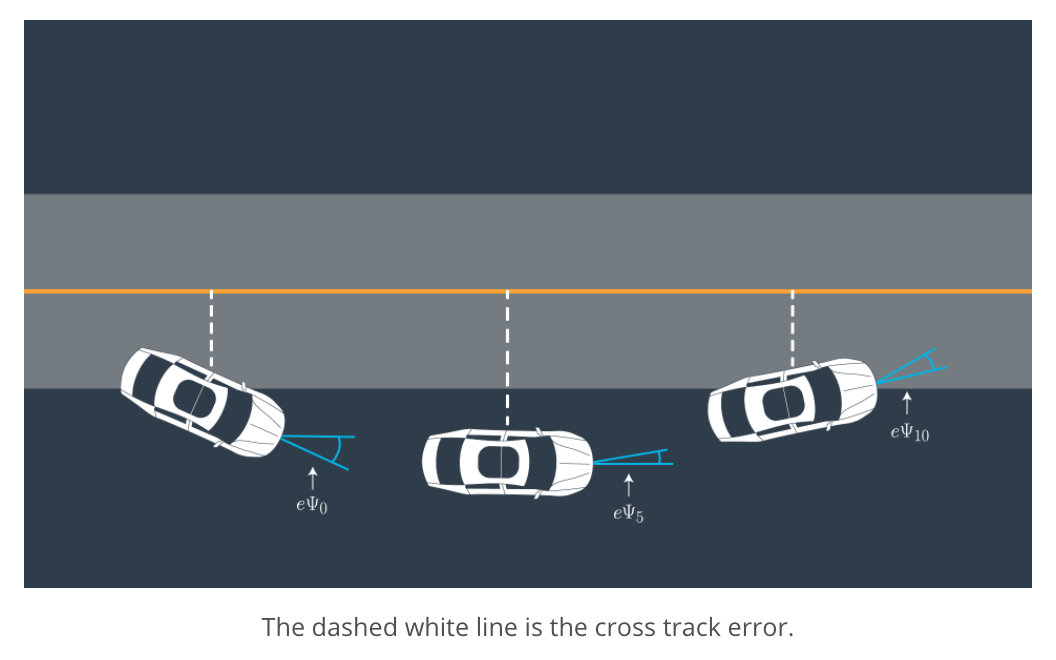
\includegraphics[width=0.75\textwidth]{errors}
    \caption{Model errors}
    \label{fig:errors}
\end{figure}
\FloatBarrier

\begin{itemize}
\item $cte$: cross track error. It corresponds to distance of vehicle from the planned trajectory (as planned by path planning module)
\item $e\Psi$: psie error is the angle difference of the vehicle trajectory with the planned trajectory (as planned by path planning module)
\end{itemize}

\textbf{The new state vector is $[x_t, y_t, \psi_t, v_t, cte_t, e\Psi_t]$.
}
\subsubsection{Kinematic Model}


\subsection{Dynamic Models}


Forces, Slip Angle, Slip ratio and Tire Models


\section{Model Predictive Control}

MPC reframes the task of following a trajectory as an optimization problem. The solution to the optimization problem is the optimal trajectory. \\

MPC involves simulating different actuator inputs, predicting the resulting trajectory and minimizing a set of constraints (or cost functions). \\ 

\textbf{Input:} a reference trajectory we want to follow \\ \\
\textbf{Constraints:}
\begin{itemize}
\item Vehicle Model
\item Comfort
\end{itemize}

\textbf{Output:} actuator commands (steering, throttling, braking ...)  \\ \\

Once we found the lowest cost trajectory, we implement the very first set of actuation commands. Then we throw away the rest of the trajectory we calculated. Instead of using the old trajectory we predicted, we take our new state and use that to calculate a new optimal trajectory. In that sense, we are constantly calculating inputs over a future horizon. That's why this approach is also called Receding Horizon Control. We constantly reevaluate the trajectory because our vehicle model is not perfect and the next predicted (or planned) state may (slightly...) differ with our prediction (in the sense of a consequence of a command sent). 


\begin{figure}[h]
    \centering
    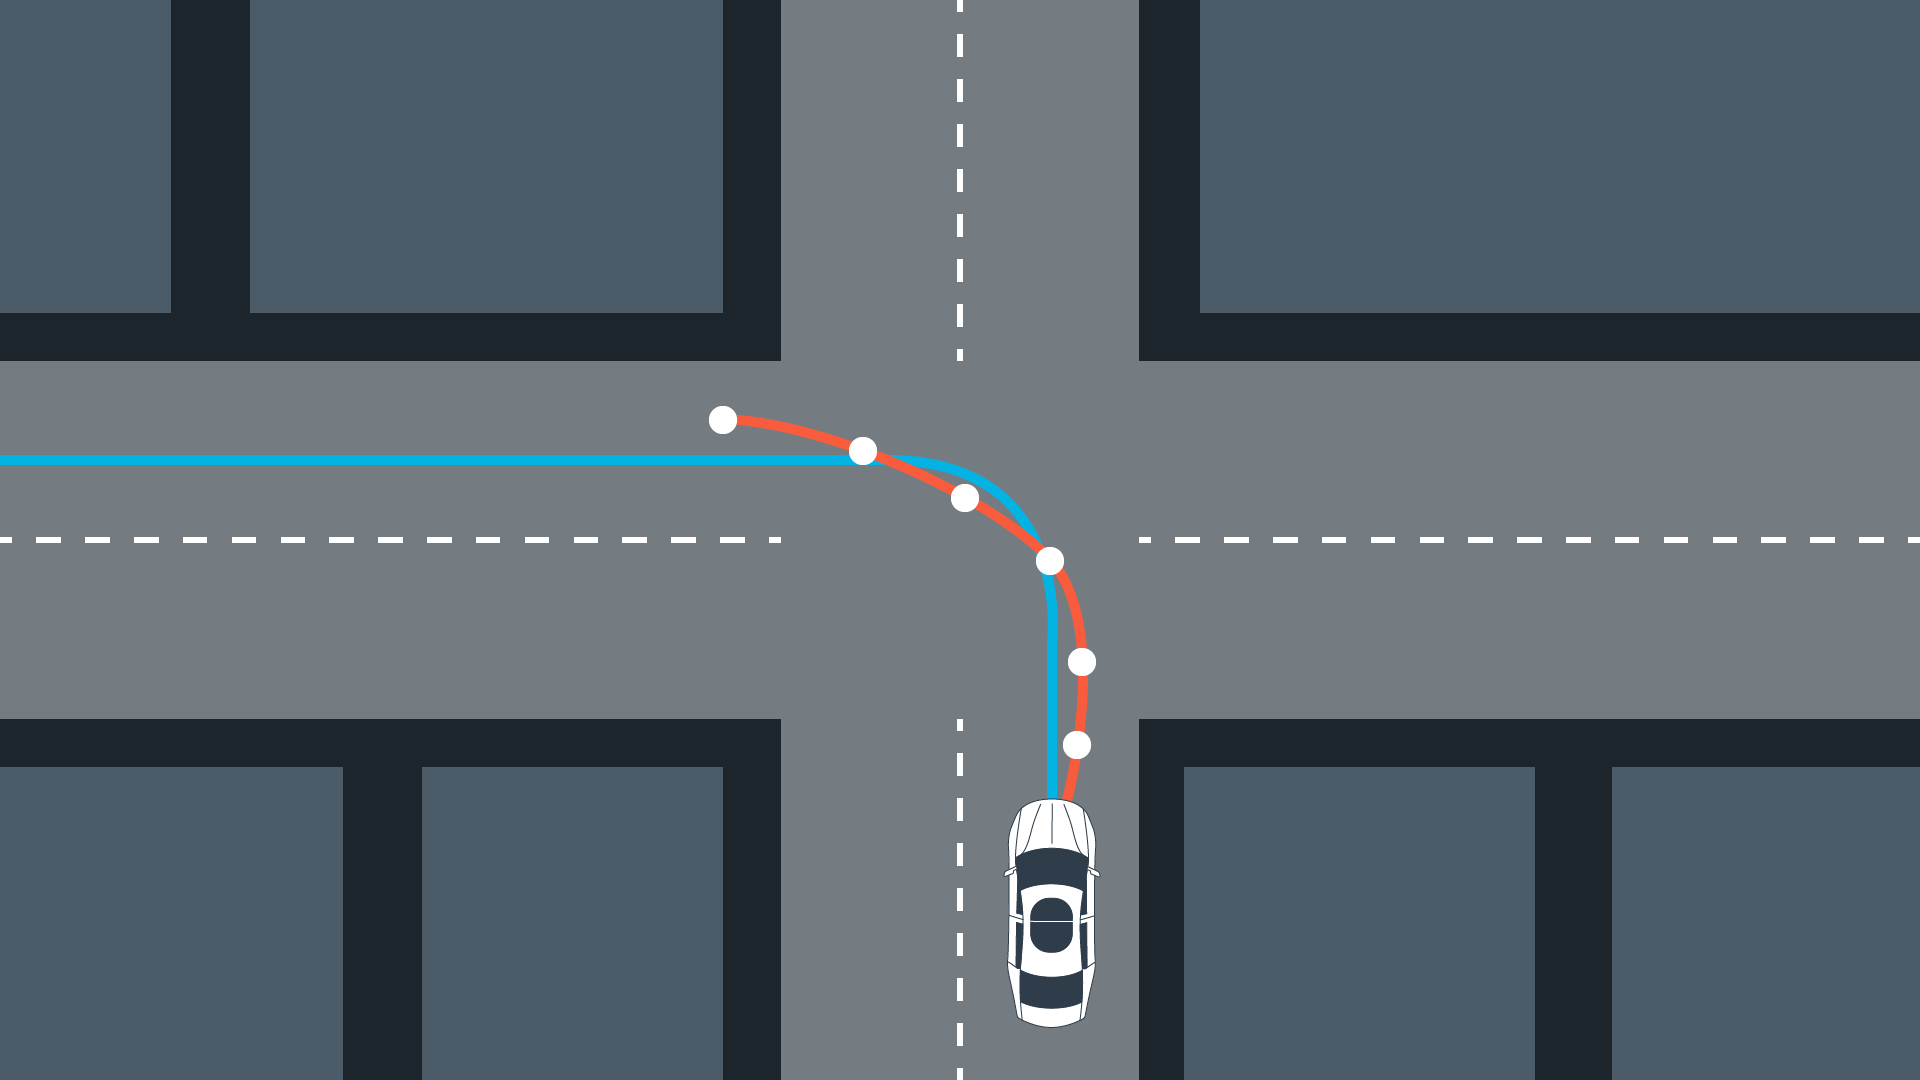
\includegraphics[width=0.5\textwidth]{minimization}
    \caption{Minimization problem}
    \label{fig:minimization}
\end{figure} 

\subsection{Optimization under constraints: cost functions}

\subsection{Timsestep length and Elapsed duration}

N=10 and dt=100 ms are used so that we are working on 1 second of data.
This is a trade-off: we need enough data visibility to ensure a good prediction, but we also have to limit the amount of computation.
In general, smaller dt gives better accuracy, but that will require higher N for given horizon (N*dt). However, increasing N will result in longer computational time which increases the latency. The most common choice of values is N=10 and dt=0.1 but anything between N=20, dt=0.05 should work.

\begin{figure}[h]
    \centering
    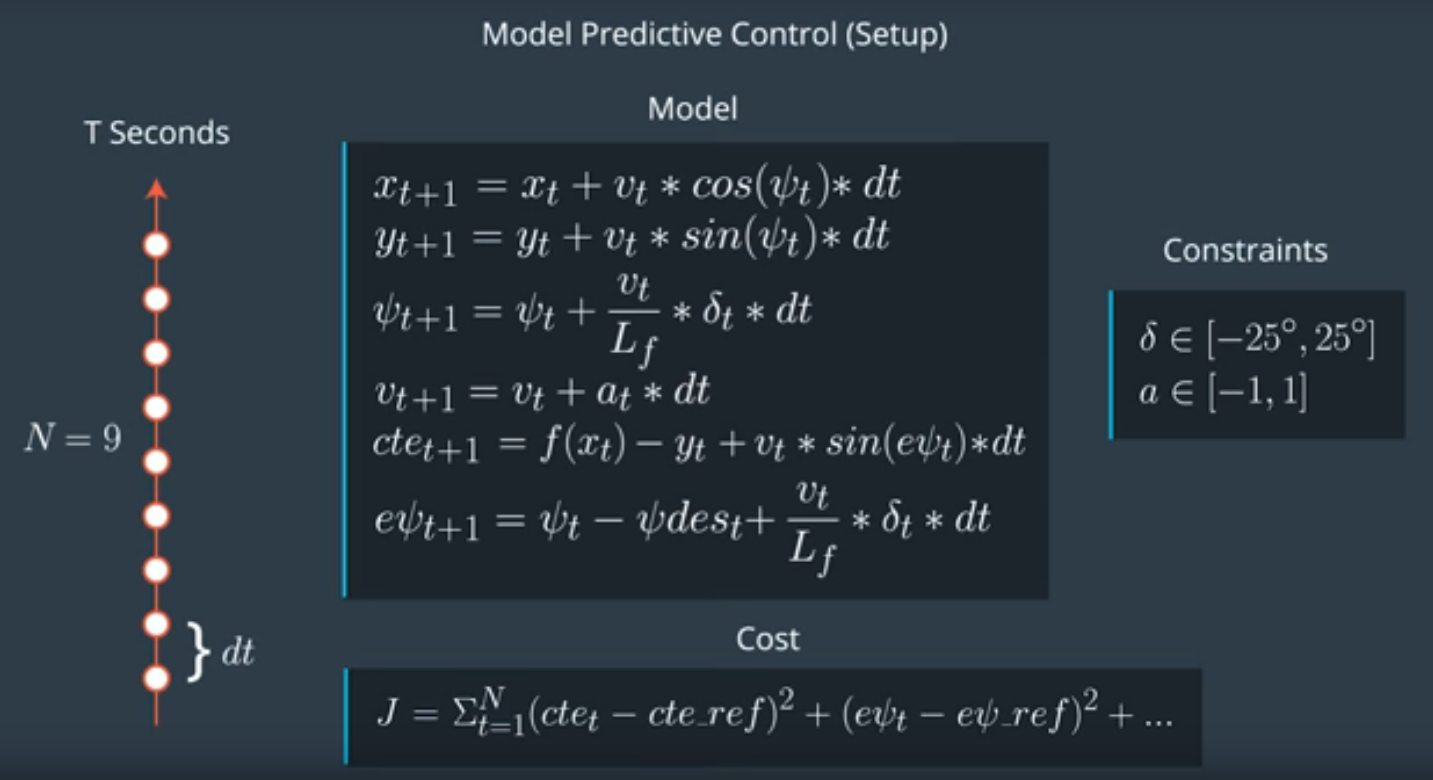
\includegraphics[width=0.75\textwidth]{solver_setup}
    \caption{Solver setup with N*dt time horizon}
    \label{fig:solver_setup}
\end{figure}

\subsection{Latency handling}


A contributing factor to latency is actuator dynamics. For example the time elapsed between when you command a steering angle to when that angle is actually achieved. This could easily be modeled by a simple dynamic system and incorporated into the vehicle model. One approach would be running a simulation using the vehicle model starting from the current state for the duration of the latency. The resulting state from the simulation is the new initial state for MPC.

Thus, MPC can deal with latency much more effectively, by explicitly taking it into account, than a PID controller.

\subsection{MPC Solver algorithm}

\begin{figure}[h]
    \centering
    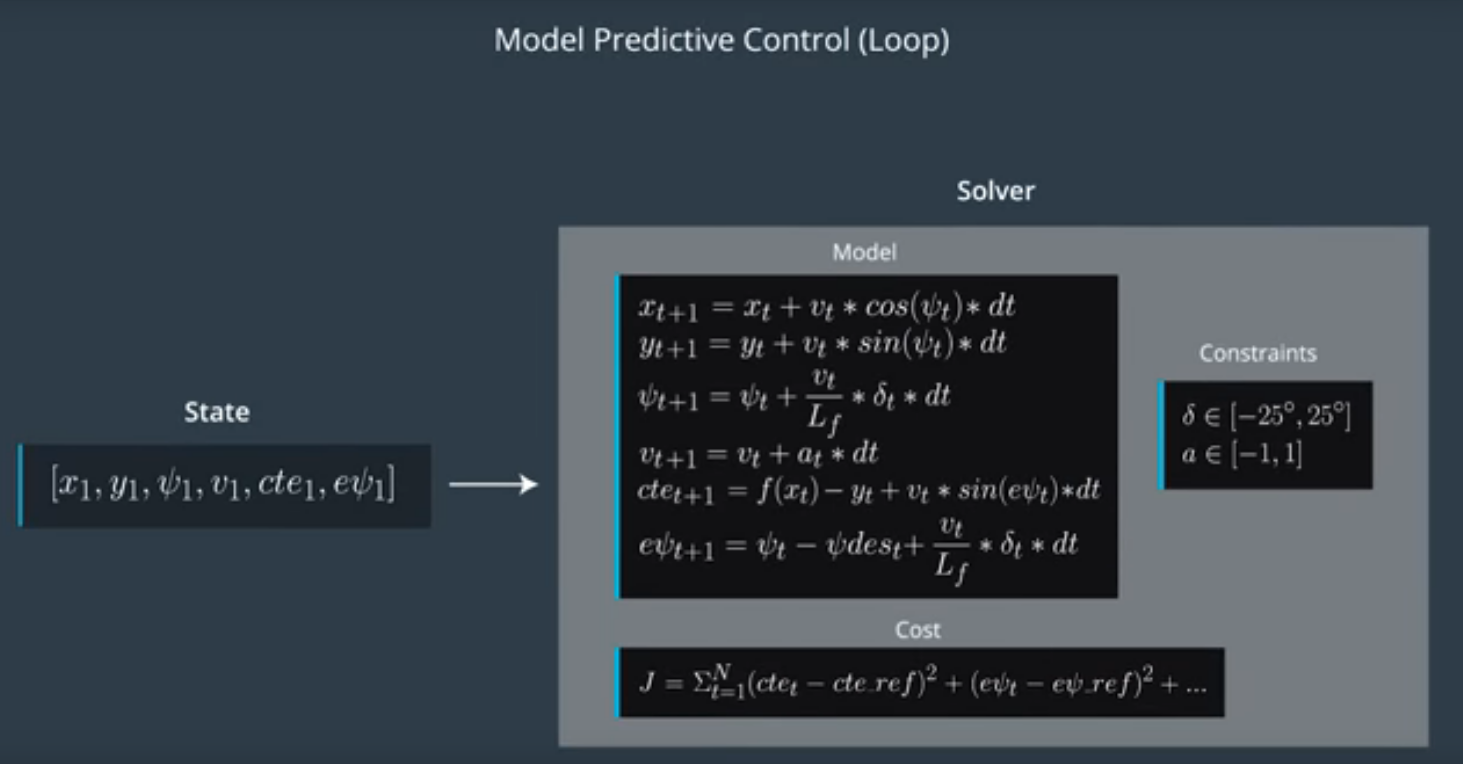
\includegraphics[width=0.75\textwidth]{solver_in}
    \caption{Solver input}
    \label{fig:solver_in}
\end{figure}

\begin{figure}[h]
    \centering
    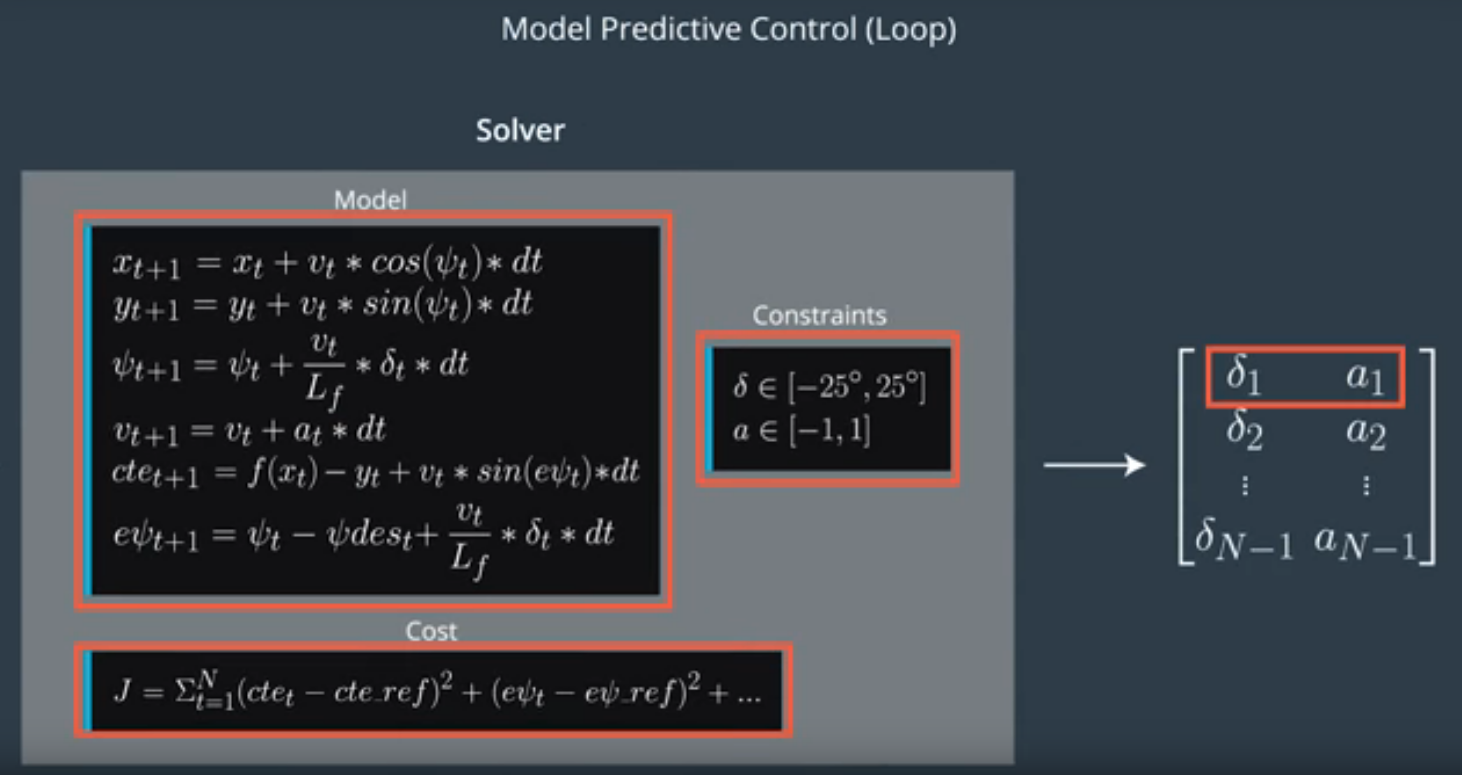
\includegraphics[width=0.75\textwidth]{solver_out}
    \caption{Solver output}
    \label{fig:solver_out}
\end{figure}

\begin{figure}[h]
    \centering
    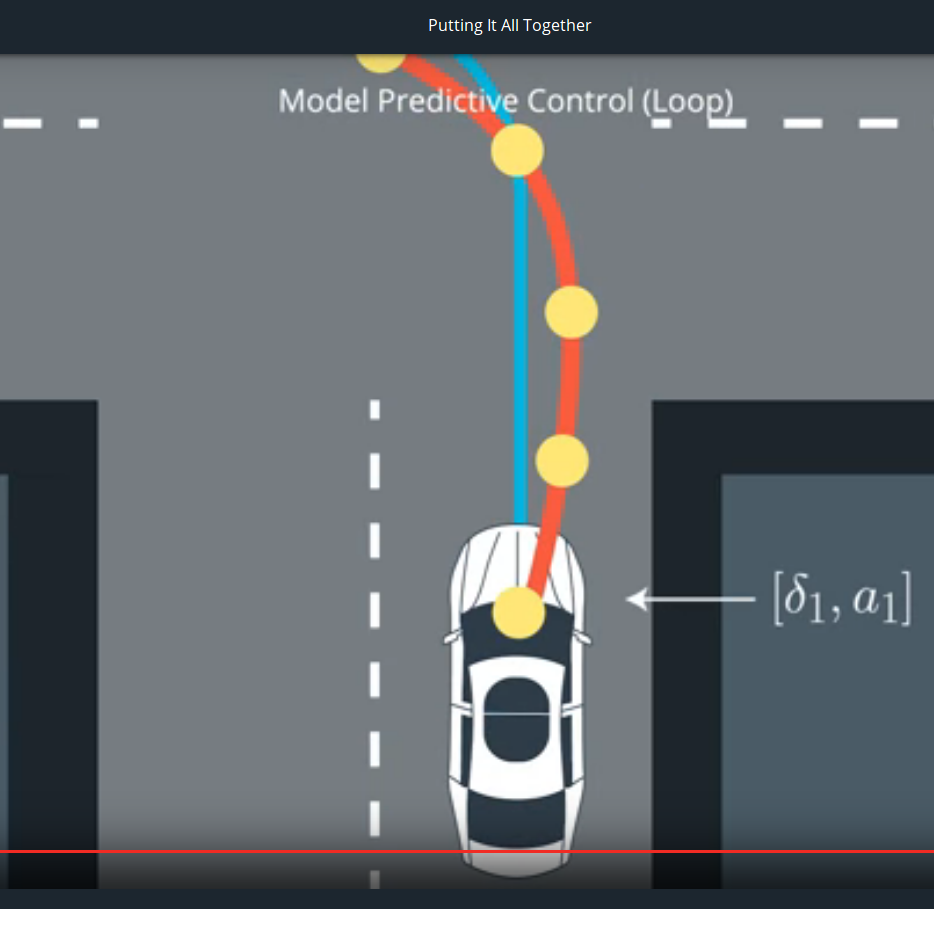
\includegraphics[width=0.5\textwidth]{solver_actuate}
    \caption{Solver actuator commands}
    \label{fig:solver_actuate}
\end{figure}

\FloatBarrier


\end{document}}